%\hskip 2.5cm
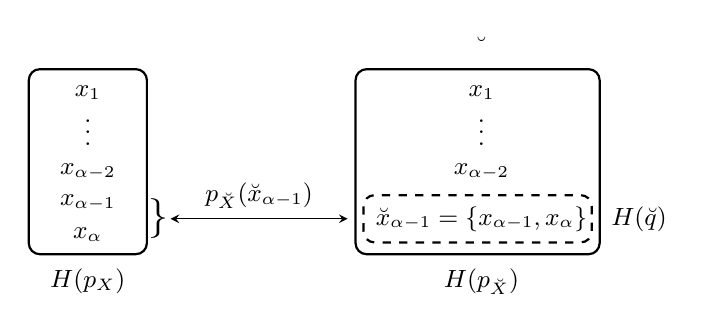
\begin{tikzpicture}
\shorthandoff{>}
%
% Ensemble \X
\draw(0,3) node{\small $\X$};
\draw(0,2.4) node{\small $x_1$};
\draw(0,2) node{\small $\vdots$};
\draw(0,1.4) node{\small $x_{\alpha-2}$};
\draw(0,1) node{\small $x_{\alpha-1}$};
\draw(0,.6) node{\small $x_{\alpha}$};
\draw(0,0) node{\small $H(p_X)$};
\draw[thick,rounded corners] (-.75,.35) rectangle (.75,2.7);
%
% Ensemble \breve{\X}
%
\draw(5,3) node{\small $\breve{\X}$};
\draw(5,2.4) node{\small $x_1$};
\draw(5,2) node{\small $\vdots$};
\draw(5,1.4) node{\small $x_{\alpha-2}$};
\draw(5,.8) node{\small $\breve{x}_{\alpha-1} = \{ x_{\alpha-1} , x_\alpha\}$};
\draw(5,0) node{\small $H(p_{\breve{X}})$};
\draw(7,.8) node{\small $H(\breve{q})$};
\draw[dashed,thick,rounded corners] (3.5,.5) rectangle (6.4,1.1);
\draw[thick,rounded corners] (3.4,.35) rectangle (6.5,2.7);
%
% juntando 2 estados VER PROBLEMA CON LA FLECHA
\draw(.9,.8) node{\Large $\}$};
\draw[>=stealth,<->] (1.05,.8)--(3.3,.8);
\draw (2.175,.8) node[above]{\small $p_{\breve{X}}(\breve{x}_{\alpha-1})$};
\end{tikzpicture}